%%%%%%%%%%%%%%%%%%%%%%%%%%%%%%%%%%%%%%%%%%%%%%%%%%%%%%%%%%%%%%%%%%%%%%%%%%%%%%%
% Chapter 'Adsorption - Water - silica gel pellet WS'
%%%%%%%%%%%%%%%%%%%%%%%%%%%%%%%%%%%%%%%%%%%%%%%%%%%%%%%%%%%%%%%%%%%%%%%%%%%%%%%
\subsection{Silica gel pellet WS}
%
%%%%%%%%%%%%%%%%%%%%%%%%%%%%%%%%%%%%%%%%%%%%%%%%%%%%%%%%%%%%%%%%%%%%%%%%%%%%%%%
%%%%%%%%%%%%%%%%%%%%%%%%%%%%%%%%%%%%%%%%%%%%%%%%%%%%%%%%%%%%%%%%%%%%%%%%%%%%%%%
\subsubsection{DubininArctan1 - ID 1}
%
\begin{tabular}[l]{|lp{11.5cm}|}
\hline
\addlinespace

\textbf{Sorbent:} & silica gel pellet \\
\textbf{Subtype:} & WS \\
\textbf{Refrigerant:} & Water \\
\textbf{Equation:} & DubininArctan1 \\
\textbf{ID:} & 1 \\
\textbf{Reference:} & Schawe, D. (2000): Theoretical and Experimental Investigations of an Adsorption Heat Pump with Heat Transfer between two Adsorbers. Dissertation. Universität Stuttgart, Stuttgart. Energietechnik. \\
\textbf{Comment:} & None \\

\addlinespace
\hline
\end{tabular}
\newline

\textbf{Properties of sorbent:}
\newline
%
\begin{longtable}[l]{lll}
\toprule
\addlinespace
\textbf{Property} & \textbf{Unit} & \textbf{Value} \\
\addlinespace
\midrule
\endhead
\bottomrule
\endfoot
\bottomrule
\endlastfoot
\addlinespace

Diameter of pore & \si{\milli\meter} & 2.50E-06\\
Surface area & \si{\square\meter\per\gram} & 650\\
Pore volume & \si{\milli\cubic\meter\per\gram} & 0.4\\
Bulk density & \si{\kilogram\per\cubic\meter} & 700\\

\addlinespace\end{longtable}

\textbf{Equation and parameters:}
\newline
%
Loading $w$ in $\si{\kilogram\per\kilogram}$ is calculated depending on pressure $p$ in $\si{\pascal}$, temperature $T$ in $\si{\kelvin}$, and vapor pressure $p_\mathrm{sat}$ in $\si{\pascal}$ by:
%
\begin{equation*}
\begin{split}
w &=& W \rho_\mathrm{sat}^{\mathrm{liq}} & \quad\text{, and} \\
W &=& \frac{a}{\Pi} \left( \arctan \left( \frac{A - b}{c} \right) + \frac{\Pi}{2}\right) + d & \quad\text{, and} \\
A &=& R T \ln \left( \nicefrac{p_\mathrm{sat}}{p} \right) & \quad\text{.} \\
\end{split}
\end{equation*}
%
The parameters of the equation are:
%
\begin{longtable}[l]{lll|lll}
\toprule
\addlinespace
\textbf{Par.} & \textbf{Unit} & \textbf{Value} &	\textbf{Par.} & \textbf{Unit} & \textbf{Value} \\
\addlinespace
\midrule
\endhead

\bottomrule
\endfoot
\bottomrule
\endlastfoot
\addlinespace

$a$ & $\si{\cubic\meter\per\kilogram}$ & 5.046468000e-04 & $c$ & $\si{\joule\per\mole}$ & -1.308650854e+03 \\
$b$ & $\si{\joule\per\mole}$ & 1.805355210e+03 & $d$ & $\si{\cubic\meter\per\kilogram}$ & 0.000000000e+00 \\

\addlinespace\end{longtable}

\textbf{Validity:}
\newline
No data on validity available!
\newline

\textbf{Visualization:}
%
\begin{figure}[!htp]
{\noindent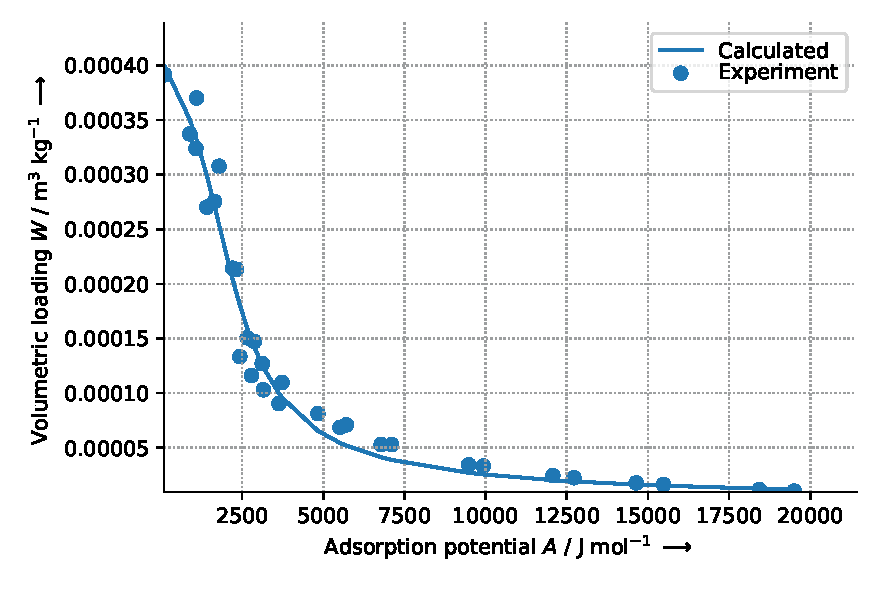
\includegraphics[height=10cm, keepaspectratio]{figs/ads/ads_Water_silica_gel_pellet_WS_DubininArctan1_1.pdf}}
\end{figure}
%

To generate the figure, the following refrigerant functions were selected:
\begin{itemize}
\item Vapor pressure: VaporPressure\_EoS1 - ID 1
\item Saturated liquid density: SaturatedLiquidDensity\_EoS1 - ID 1
\end{itemize}

The uncertainity of the experimental data is:
\begin{itemize}
\item Data source $\,\to\,$ Data was taken from figure
\item Loading, absolute, in $\si{\kilogram\per\kilogram}$ $\,\to\,$ 0.000001
\end{itemize}

The mean absolute percentage error (MAPE) between the experimental and calculated data results in 13.65\%.
\FloatBarrier
\newpage
%%%%%%%%%%%%%%%%%%%%%%%%%%%%%%%%%%%%%%%%%%%%%%%%%%%%%%%%%%%%%%%%%%%%%%%%%%%%%%%
